\chapter{Lập trình hệ thống nhúng trong Rust}
\section{Điều khiển vi điều khiển}
Trước hết, ta cần phải hiểu về cách để điều khiển một vi điều khiển.
Ta thực hiện điều khiển vi điều khiển bằng cách điều khiển (đọc hoặc viết) các register trên vi điều khiển.
Các register trên vi điều khiển thường là memory mapped, điều này có nghĩa là ta điều khiển các register này bằng cách viết các byte vào các địa chỉ bộ nhớ nhất định, và sau đó vi điều khiển sẽ đọc các byte này và sau đó điều khiển các ngoại vi của nó.

Để có được các thông số về các byte viết vào các vùng nhớ này có dạng như thế nào, viết vào vùng nhớ nào, địa chỉ là bao nhiêu ta phải đọc datasheet do nhà sản xuất các vi điều khiển này cung cấp.

Các datasheet được nhà sản xuất cung cấp này thường rất dài và chứa đựng rất nhiều thông tin về sản phẩm, datasheet của EK-TM4C123GH6PM có độ dài tới 1410 trang! \cite{tivac_datasheet}.

Để minh họa, tôi xin đưa ra một ví dụ cụ thể là điều khiển kích hoạt clock cho GPIO trên kit Tiva C EK-TM4C123GH6PM, sau đó kích hoạt các GPIO này bằng cách ghi trực tiếp vào các register.
Trước hết, ta cần phải xác định được các thông số cần phải thay đổi. Ở ví dụ này, các thông số đó được trình bày trong datasheet ở trang 340.
\begin{figure}[ht]
\centering
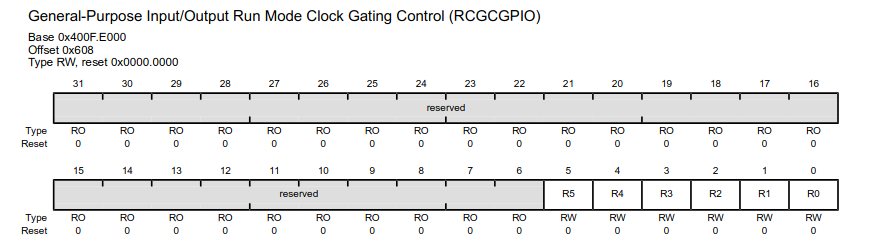
\includegraphics[scale=0.5]{images/tivac_datasheet_example.png}
\caption{Các thông số về RCGCGPIO của EK-TM4C123GH6PM ở trang 340}
\end{figure}

Dựa vào thông số này, nếu ta muốn kích hoạt clock cho GPIOF, và sau đó kích hoạt quyền ghi vào GPIOF ta sẽ viết một đoạn code C như sau:
\begin{listing}[ht]
\begin{ccode}
#include "TM4C123GH6PM.h"
SYSCTL->RCGCGPIO |= 0x20; // kich hoat clock cho GPIOF
GPIOF->LOCK = 0x4C4F434B; // unlockGPIOCR register
\end{ccode}
\caption{Ví dụ ghi trực tiếp vào các register sử dụng C}
\end{listing}

Các thao tác đọc ghi các thanh ghi này là các thao tác được cho là cấp thấp (low-level), thường chỉ các ngôn ngữ cấp thấp như C/C++ mới có thể thực hiện các thao tác này.
Các ngôn ngữ cấp cao thường không thể thực hiện trực tiếp các thao tác này, làm cho các ngôn ngữ này không thể lập trình nhúng được.
Rust là một ngôn ngữ cấp thấp,  ta cũng có thể thực hiện các thao tác tương tự như vậy nếu cần thiết.
Sau đây, tôi đưa ra một ví dụ về sử dụng Rust để thực hiện một thao tác tương tự trên một vi điều khiển STM32F1 để chứng minh điều này.
\begin{listing}[ht]
\begin{rustcode}
const GPIO_START: usize = 0x4001_1000;
const CRH_OFFSET: usize = 0x04;
const OUTPUT_MODE: u32 = 0b01;
const PUSH_PULL: u32 = 0b10;

unsafe {
    *((GPIOC_START + CRH_OFFSET) as *mut u32) = (OUTPUT_MODE << 20) | (PUSH_PULL << 22);
}
\end{rustcode}
\caption{Ví dụ ghi trực tiếp vào các register sử dụng Rust}
\end{listing}

Có thể dễ dàng nhận thấy rằng cách này rất khó viết, khó hiểu, tốn thời gian đọc datasheet và cực kỳ thiếu an toàn.
Để giải quyết các vấn đề này ta thường sử dụng các thư viện để abstract công việc này.
\section{Các thư viện abstract đề điều khiển vi điều khiển}
\subsection{Các thư viện abstract trong C}
Các thư viện thực hiện công việc abstract này trong C/C++ thường được cung cấp sẵn bởi nhà sản xuất.
Ta chỉ việc tải xuống các thư viện này, liên kết nó với phần mềm là có thể sử dụng được.
Ví dụ, để điều khiển EK-TM4C123GH6PM ta có thể tải xuống thư viện TivaWare \cite{tivac_tivaware} và sử dụng nó.
Sau khi được abstract, một chương trình khởi động port GPIO cũng như thiết lập cho nó có thể tương tự như sau:
\begin{listing}[ht]
\begin{ccode}
void setup_GPIOs()
{
     delay_ms(2000);
     GPIO_Clk_Enable(&GPIO_PORTF);
     GPIO_Config(&GPIO_PORTF,
                 (_GPIO_PINMASK_1 | _GPIO_PINMASK_2 | _GPIO_PINMASK_3),
                 _GPIO_DIR_OUTPUT,
                 (_GPIO_CFG_DIGITAL_ENABLE | _GPIO_CFG_DRIVE_8mA),
                 _GPIO_PINCODE_NONE);
}
\end{ccode}
\caption{Ví dụ về sử dụng một thư viện abstract trong C}
\end{listing}

Có thể thấy rằng, khi sử dụng các thư viện này ta có thể điều khiển các vi điều khiển một cách tương đối dễ dàng và an toàn.
Tuy nhiên, mặc dù đã được abstract, để có thể sử dụng điều khiển vi điều khiển một cách thích hợp ta vẫn phải đọc datasheet.
Ngoài ra, cách này có một nhược điểm lớn đó là các thư viện abstract này là platform-specific, điều này có nghĩa là chúng ta không thể sử dụng được thư viện này cho các các vi điều khiển khác.
Nếu ta muốn sử dụng một thư viện driver ngoài để tương tác với thiết bị ngoài, ta phải tự định nghĩa lại các thông số trong các thư viện này thì mới có thể sử dụng được nó.
Đây là một nhược điểm lớn đối với người lập trình nhúng, vì nếu muốn sử dụng nhiều vi điều khiển khác nhau thì ta phải học các thư viện viện khác nhau.

\subsection{Các thư viện abstract trong Rust}
Các thư viện thực hiện việc abstract này trong Rust được gọi là Peripheral Access Crates (PAC).
Vì các nhà sản xuất vi điều khiển không cung cấp sẵn các PAC nên người lập trình nhúng của Rust phải tự viết các thư viện này.
Tuy nhiên, việc viết các thư viện này là điều cực kỳ tốn công sức và dễ bị lỗi nên các nhà phát triển lập trình nhúng của Rust đi theo một hướng khác đó là sử dụng các file SVD được cung cấp sẵn bởi nhà sản xuất.
Các nhà sản xuất vi điều khiển ngoài việc cung cấp các file datasheet cho sản phẩm của mình thì thường còn cung cấp thêm các file SVD.
Các file SVD này mô tả các chức năng của vi điều khiển, các ngoại vi của nó, v.v.. theo các định dạng dành cho máy tính (như XML).
Các nhà phát triển lập trình nhúng của Rust đã thực hiện viết một chương trình là \mintinline{bash}{svd2rust} để thực tạo ra các crates (thư viện của Rust) một cách tự động từ các file SVD này.
Từ kết quả thu được, cộng thêm công việc sửa lại các artifact từ kết quả nếu có,
ta thu được các thư viện abstract này một cách tự động.
Ngoài ra, vì hệ thống ownership của Rust được compiler kiểm tra lúc biên dịch nên khi sử dụng các thư viện này, chúng ta cũng được hưởng lợi từ hệ thống ownership này!
Một ví dụ ở đây về lợi ích của hệ thống ownership là ta không thể thiết lập clock cho vi điều khiển nhiều lần.

Khi sử dụng PAC, ta có thể viết mã thực hiện công việc khởi động GPIO một cách dễ dàng hơn.
\begin{listing}[ht]
\begin{rustcode}
startup_gpio();
dp.GPIOC.crh.modify(|_r, w| {
    w.mode13().output()
     .cnf13().push_pull()
});
\end{rustcode}
\caption{Ví dụ về sử dụng một PAC trong Rust}
\end{listing}

Có thể thấy rằng, sử dụng PAC ta có thể viết các mã tương đối cao hơn như C mà vẫn không mất đi hiệu suất (zero-cost abstraction), an toàn hơn, cũng như được hưởng lợi từ hệ thống ownership của Rust.

Để giải quyết vấn đề về platform-specific, Rust đi theo một hướng khác.
Tuy nhiên, cũng như việc sử dụng các thư viện abstract trong C/C++, sử dụng PAC vẫn là platform-specific vì mỗi vi điều khiển sẽ có một PAC khác nhau.
Ngoài ra, mặc dù mã đã an toàn hơn (không trực tiếp sử dụng unsafe mà abstract qua PAC), tuy nhiên các lỗi về logic vẫn không được giải quyết.
Ví dụ, nếu ta không khởi động gpio \mintinline{bash}{startup_gpio();} mà trực tiếp thiết lập GPIO thì mã sẽ vẫn được biên dịch, tuy nhiên đến runtime thì ta mới phát hiện lỗi vì vi điều khiển không chạy!
Compiler không thể biết được ta có thực hiện công việc khởi động hệ thống có đúng hay không, mà nó chỉ có thể xác định được ta sử dụng các hàm tương tác với PAC đúng hay không.

\subsection{Hardware Abstraction Layer (HAL)}
Để giải quyết vấn đề này, Rust chọn cách là tiếp tục abstract PAC thành Hardware Abstraction Layer (HAL).
Trong C, ta cũng sử dụng các HAL để tương tác với vi điều khiển, nhưng trong Rust các HAL thường cao hơn các HAL trong C.
Khi sử dụng HAL của Rust, mã viết ra thường có cảm giác tương đương với mức độ abstraction trong lập trình arduino.
Ví dụ, khi ta sử dụng HAL \mintinline{bash}{stm32f1xx\_hal} để tương tác với vi điều khiển STM32F1 để khởi động GPIO, mã Rust sẽ được viết như sau:
\begin{listing}[ht]
\begin{rustcode}
let mut rcc = dp.RCC.constrain();
let mut gpioc = dp.GPIOC.split(&mut rcc.apb2);
let mut led = gpioc.pc13.into_push_pull_output(crh);
led.set_high();
\end{rustcode}
\caption{Ví dụ về sử dụng một PAC trong Rust}
\end{listing}

Giải thích qua mã:

Ở dòng 1, ta tạo một struct gồm các ngoại vi cơ bản (tương tự như \mintinline{bash}{startup_gpio}) để có thể sử dụng với HAL, ta làm cách này bằng cách sử dụng hàm \mintinline{bash}{constrain()}.
Sau đó để thiết lập GPIO, ta mượn struct này để thực hiện thiết lập GPIO bằng hàm \mintinline{bash}{split()}, một điểm lưu ý ở đây là muốn khởi tạo GPIO sử dụng HAL ta bắt buộc phải mượn struct RCC đã khởi tạo.
Nếu ví như ta không thể mượn được struct RCC, điều này có nghĩa là việc khởi chạy các ngoại vi bị lỗi.
Compiler có thể kiểm tra việc này lúc biên dịch và sẽ báo lỗi, tránh được việc tới runtime mới phát hiện ra lỗi của hệ thống.
Tương tự, ta tiếp tục mượn struct GPIOC để thiết lập LED (pin 13), và ta thiết lập nó ở chế độ push pull output.
Sau đó, để bật LED, ta chỉ việc sử dụng hàm \mintinline{bash}{set_high()}, có một điểm cần lưu ý ở đây là nếu ta không thiết lập pin ở chế độ output thì ta sẽ không có hàm \mintinline{bash}{set_high()}, đảm bảo cho an toàn nếu người lập trình thiết lập hệ thống sai.

Sử dụng HAL như cách này, ta có một interface với hệ thống ở cấp cao, dễ dàng viết mã, và đảm bảo được an toàn ngay từ lúc biên dịch.
Ngoài ra, nếu các HAL được viết tốt, ta hoàn toàn có thể dựa vào tài liệu hướng dẫn của HAL thay vì đọc datasheet!

\subsection{Các thiết bị ngoài}
Bước tiếp theo để lập trình một hệ thống nhúng là tương tác với các thiết bị bên ngoài.
Ở đây, tôi sẽ đưa ví dụ về cách sử dụng HAL để tương tác với cảm biến nhiệt độ, độ ẩm AHT20 \cite{aht20_datasheet}.
Đây là một HAL thực tế làm driver để điều khiển AHT20 trong Rust được viết bởi các nhà phát triển lập trình nhúng \cite{hal_aht20}.

Ví dụ \ref{code:rust_hal_aht20_setup} sau đây là mã để thiết lập một thiết bị AHT20.

\begin{figure}[ht]
\centering
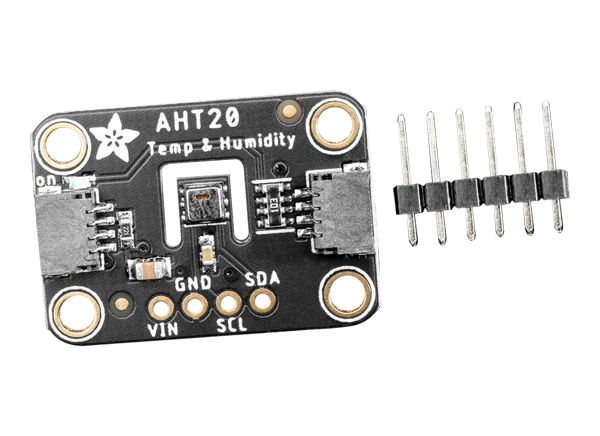
\includegraphics[scale=0.5]{images/aht20.png}
\caption{AHT20 Temperature, Humidity Sensor}
\end{figure}

\clearpage
\begin{listing}[ht]
\begin{rustcode}
pub fn new(i2c: I2C, delay: D) -> Result<Self, Error<E>> {
    let mut dev = Self {
        i2c: i2c,
        delay: delay,
    };

    dev.reset()?;

    dev.calibrate()?;

    Ok(dev)
}
pub fn calibrate(&mut self) -> Result<(), Error<E>> {
    // Send calibrate command
    self.i2c.write(I2C_ADDRESS, &[0xE1, 0x08, 0x00])?;

    // Wait until not busy
    while self.status()?.contains(StatusFlags::BUSY) {
        self.delay.delay_ms(10);
    }

    // Confirm sensor is calibrated
    if !self.status()?.contains(StatusFlags::CALIBRATION_ENABLE) {
        return Err(Error::Uncalibrated);
    }

    Ok(())
}
\end{rustcode}
\caption{Ví dụ về sử dụng HAL để viết driver cho thiết bị ngoài trong Rust}
\label{code:rust_hal_aht20_setup}
\end{listing}

Để sử dụng HAL, ta thực thao tác đơn giản:

\begin{listing}[ht]
\begin{rustcode}
let mut dev = Aht20::new(i2c, hal::Delay).unwrap();
let (h, t) = dev.read().unwrap(); // h = humidity, t = temperature
\end{rustcode}
\caption{Ví dụ về sử dụng driver HAL để tương tác thiết bị ngoài trong Rust}
\end{listing}

Có thể thấy rằng, sử dụng HAL, ta có thể viết các mã ở mức rất cao, cực kỳ tiện lợi.
Các driver sử dụng type system của Rust để đảm bảo rằng các thiết bị được thiết lập đúng
(nếu thiết lập I\textsuperscript{2}C sai thì sẽ không thể thiết lập được thiết bị AHT20).
Hệ thống ownership đảm bảo rằng các pin cũng như các ngoại vi hệ thống như I\textsuperscript{2}C không bị dùng chung ở bất cứ thời điểm nào.

Tuy nhiên, ta vẫn có thể dễ dàng nhận ra nhiều nhược điểm của HAL.
Một vài nhược điểm lớn có thể được nêu ra như:

\begin{itemize}
    \item Toàn bộ những HAL này được viết thủ công để abstract PAC.
        Không có HAL nào được viết tự động từ PAC cả.
        Điều này dẫn đến hai vấn đề khác là chất lượng của các HAL này phụ thuộc phần lớn vào người thiết kế các HAL này.
        Một vấn đề khác là vì viết các HAL là công việc thủ công nên không phải toàn bộ các chức năng của vi xử lý được định nghĩa trong PAC sẽ có lớp abstraction HAL.
    \item Vì mỗi HAL sẽ có một API để tương tác với vi điều khiển khác nhau nên người dùng thiết kế hệ thống nhúng sử dụng nhiều vi điều khiển khác nhau thì họ vẫn phải học cách sử dụng nhiều HAL khác nhau.
    \item Đến đây, ta vẫn chưa giải quyết được vấn đề về platform specific. Nếu muốn crate driver tương tác với thiết bị ngoài hỗ trợ cho vi xử lý nào đó, người lập trình HAL phải tự viết một HAL riêng cho các driver này. \label{list:hal_prob}
\end{itemize}

\subsection{Embedded HAL}
Để giải quyết vấn đề này, các nhà lập trình nhúng của Rust dựa trên một tính năng có sẵn trong Rust đó là sử dụng \mintinline{bash}{traits} để tái sử dụng lại các thuộc tính được định nghĩa sẵn.
Crate dùng để định nghĩa các trait cho ngoại vi thông dụng (như GPIO, Timer, SPI, UART, v.v..) này được gọi là \mintinline{bash}{Embedded HAL} \cite{embedded_hal}.

Sau khi có được các trait định nghĩa từ Embedded HAL, các nhà lập trình nhúng viết HAL cho các vi điều khiển riêng biệt tái sử dụng lại các trait này để viết HAL cho vi điều khiển của mình.
Sau khi hoàn thành, những người viết driver cho các thiết bị ngoài trong Rust chỉ việc tái sử dụng lại các trait được định nghĩa trước này.
Bất cứ HAL cho các vi điều khiển nào mà đã tái sử dụng các trait này thì chắc chắn driver sẽ hoạt động cho vi điều khiển đó mà không cần phải chỉnh sửa lại crate driver.
Ta chỉ việc viết driver một lần duy nhất và toàn bộ tất cả các HAL cho vi điều khiển đều có thể sử dụng driver này.
Đây chính là điểm then chốt trong hệ sinh thái lập trình nhúng của Rust.

Để xem một ví dụ, ta xem lại ví dụ về driver AHT20 của Rust (ví dụ \ref{code:rust_hal_aht20_setup}).
Ở đây, tôi đã thêm phần tái sử dụng trait trong ví dụ mới này.
Có thể thấy rằng, driver này đã tái sử dụng hai trait từ Embedded HAL đó là \mintinline{bash}{delay} và \mintinline{bash}{i2c}.
Điều này có nghĩa là bất cứ HAL cho vi điều khiển nào cũng tái sử dụng hai trait này từ Embedded HAL đều có thể sử dụng crate driver này một cách trực tiếp mà không cần thay đổ bất cứ thông số nào.
\begin{listing}[ht]
\begin{rustcode}
use embedded_hal::blocking::{delay::DelayMs, i2c::{Write, WriteRead}};
pub fn new(i2c: I2C, delay: D) -> Result<Self, Error<E>> {
\end{rustcode}
\caption{Ví dụ về tái sử dụng trait để viết driver trong Rust}
\end{listing}

Đến đây, ta đã có được một hệ thống hoàn chỉnh, sẵn sàng để áp dụng vào viết các hệ thống nhúng một cách nhanh gọn, an toàn và dễ dàng.
Ở chương tiếp theo, tôi đi vào thực hiện áp dụng Rust để viết một số hệ thống nhúng và chạy các chương trình này trên một vi điều khiển thực để minh họa cách chúng ta có thể áp dụng Rust để lập trình nhúng như thế nào.
